\documentclass[fontsize=11pt,a5paper,twoside]{memoir}
\usepackage[
  top=2cm,bottom=2cm,
  inner=1.75cm,
  outer=1.25cm,
  textwidth=13cm
]{geometry}
\strictpagecheck

\usepackage[utf8]{inputenc}

\usepackage[german]{babel}
\hyphenation{Mi-ne-ral-was-ser}

\usepackage{graphicx} % Required to include images
\usepackage{listingsutf8}
\usepackage{xfrac}
\usepackage{marvosym}
\usepackage{lettrine}
\usepackage{hyperref}
\usepackage{hyphenat}

\usepackage{almendra}
\usepackage[T1]{fontenc}

\usepackage[hang,flushmargin,multiple]{footmisc}

% latin terms displayed in palatino font
\DeclareFixedFont{\lattext}{T1}{ppl}{m}{n}{10}

% custom footnote or common font
\DeclareFixedFont{\cftext}{T1}{ppl}{m}{n}{8}
\DeclareFixedFont{\cfetext}{T1}{ppl}{m}{it}{8}
\DeclareFixedFont{\cfbtext}{T1}{ppl}{bx}{n}{8}

\newenvironment{addenumfont}{\cftext}{\par}
\newenvironment{commonfont}{\cftext}{\par}

\usepackage[perpage]{manyfoot}
\DeclareNewFootnote{A}[roman]
\DeclareNewFootnote{B}[arabic]

\usepackage{fancyhdr}
\pagestyle{fancy}
\renewcommand{\headrulewidth}{0pt}

\fancyhead[L,R,C]{}
\fancyfoot[L,R,C]{}

\title{laugensalzige Luftsauerwasser}
\author{A. v. Stipriaan Luïsçius, der Arzneiwissenschaftler\\Dr. und Prof. der Chemie zu Delft.}

\date{1799}

% TITLE PAGE

\renewcommand{\maketitlehooka}{
\centering
Art und Weise,
\vfill
\emph{um das}
}
\renewcommand{\maketitlehookb}{
({\lattext Aqua mephitica alcalina})
\vfill\vfill
mit leichter Mühe, und ohne große Kosten vermittelst des
\vfill\vfill
{\LARGE Fachinger Mineralwassers}
\vfill\vfill
zuzubereiten.
\vfill\vfill\vfill
\emph{Von}
}
% hier fügt \maketitle den Author ein
\renewcommand{\maketitlehookc}{
\vfill
\emph{Nebst}
\vfill
einer Nachricht an das Publikum über die vorzüglichen Heilkräfte des Fachinger Mineralwassers,
\vfill
von Dr. F. Diel, Physicus zu Dietz\\und Arzt im Baad Embs.
\vfill\vfill\vfill\vfill\vfill\vfill
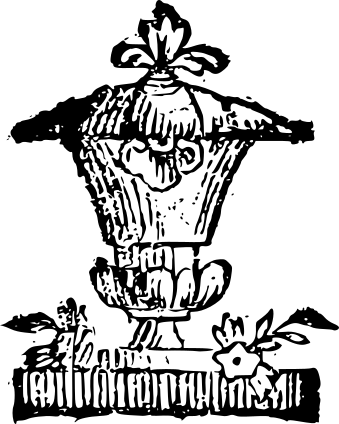
\includegraphics[width=2cm]{figures/path75}\\[.5cm]
\vfill

\begin{minipage}{4cm}
  \centering
  \hrulefill\\
\end{minipage}

\vfill
}

\newcommand{\fnadda}{, siehe Anhang \cfetext{Zu den Maßeinheiten}}

\begin{document}
\pagenumbering{gobble}

\maketitle

\newpage
\mbox{}
\newpage

\pagenumbering{arabic}
\setcounter{page}{3}
\fancyhead[C]{=\kern-0.14em=\kern-0.14em=\kern-0.14em=\kern-0.14em=\kern-0.14em=\kern-0.14em=\kern-0.14em=\kern-0.14em=\kern-0.14em=\kern-0.14em=\kern-0.14em=\kern-0.14em=\kern-0.14em=\kern-0.14em=\kern-0.14em=\kern-0.14em=\kern-0.14em=\kern-0.14em=\kern-0.14em=\kern-0.14em=\kern-0.14em=\kern-0.14em=\kern-0.14em=\kern-0.14em=\kern-0.14em=\kern-0.14em=\kern-0.14em=\kern-0.14em=\kern-0.14em=\kern-0.14em=\kern-0.14em=\kern-0.14em=\kern-0.14em=\kern-0.14em=\kern-0.14em=\kern-0.14em=\kern-0.14em=\kern-0.14em=\kern-0.14em=\kern-0.14em=\kern-0.14em=\kern-0.14em=\kern-0.14em=\kern-0.14em=\kern-0.14em=\kern-0.14em=\kern-0.14em=\kern-0.14em=\kern-0.14em=\kern-0.14em=\kern-0.14em=\kern-0.14em=\kern-0.14em=\kern-0.14em=\kern-0.14em=\kern-0.14em=\kern-0.14em=\kern-0.14em=\kern-0.14em=\kern-0.14em=} % Page numbering for center header

\null
\vfill

\noindent
\emph{Wie man das laugensalzige Luftsauerwasser
({\lattext Aqua mephitica alcalina})
mit leichter Mühe und ohne große Kosten zubereiten könne,
zeigt Hr. Prof. A. v. Stipriaan Luïsçius zu Delft
in einem Aufsatze, den er in die holländische Zeitung:
{\lattext Nieuwe allgemeene Konst - en Letter Bode}
am 10. August 1798 einrücken ließ,
und den man hier in einer freien Übersetzung
zur Kenntnis des deutschen Publikums bringt.}\\

\vspace{5em}

\lettrine{D}a ich mich verpflichtet finde,
sagt Hr. v. Stipriaan Luïsçius, jede Gelegenheit zu ergreifen,
um den Wert des laugessalzigen Luft-Sauerwassers,
wegen seiner in der Arzneiwissenschaft wesentlichen Dienste,
welche ich nebst anderen jeden Tag beobachte,
mehr und mehr zu erheben, näher bekannt zu machen,
und dessen Anschaffung zu erleichtern;
so habe ich nicht unschicklich geachtet,
mir für Nachfolgendes eine kleine Stelle
in diesem nützlichen Wochenblatt auszubitten.\\

Es wird nicht nötig sein,
die Tugenden von diesem Mittel aufs Neue durch Beispiele zu bestätigen,
welches schon genügsam in verschiedenen Werken der Scheick Bibliothek%
\footnoteA{Zu Delft bei Koelofswaart.}
und in dem Bericht von William Falconer%
\footnoteA{Aus dem Englischen übersetzt
von Dr. du Clour zu Leyden bei Herding 1796.}
geschehen, und den meisten unseren Landsleuten bekannt ist.
Ich werde nun so viel davon bemerken, daß es der guten Erwartung,
die man nach so vieler Erhebung natürlich davon haben muß,
entspreche, wo nicht übertreffe,
und daß es unter denjenigen Mitteln eine Stelle verdiene,
die, wie sie gehörig und zur rechten Zeit angewendet werden,
beinahe jederzeit den besten Erfolg haben müssen.\\

So wie die China%
\footnoteB{\cftext Chinarinde} bei den Wechselfiebern,
die Brechwurzel in einigen Arten von Rhur%
\footnoteB{\cftext schwerer Durchfall},
und die Rhababer in Verschleimung der ersten Wege oder der Gedärme wirkt,
eben so heilsam und sicher wirkt und unser Mittel auf Steinschmerzen,
die von sandigen, griesigen oder kristallförmigen Stoffen%
\footnoteB{\cftext Nierensteine}
entstehen.\\

Da nun, ungeachtet der Chemie solche starke Fortschritte gemacht hat,
unser bezwecktes Wasser gehörig zusammen zu setzen,
doch noch für Viele ein unbegreiflicher Handgriff ist;
so habe ich geglaubt, dem Publikum einen wesentlichen Dienst zu erweisen,
dasselbe mit einer leichten Zusammensetzung dieses Wassers
hierdurch bekannter zu machen.\\

Schon im Jahre 1793 gab einer meiner Freunde einen Vorschlag
zur leichten Verfertigung des mit Luftsäure gesättigten Laugensalzes,
und riet zu dem Ende zwei Quentchen Sodasalz%
\footnoteB{\cftext 7,6 Gramm Natron\fnadda{}}
in einer Unze Wasser aufzulösen,
und von dieser Auflösung jedes Mal
einen Löffel in gutem Mineralwasser einzunehmen.
Hierzu schlug er besonders Selteser, Lamscheider, Pyrmonter
oder  Dryburger Wasser vor.\\

Da ich nun glaube, in der Wahl des Salzes,
besonders aber in den Sorten des Wassers
eine merkliche Verbesserung hervorbringen zu können;
so dient noch folgendes zur Vorschrift:\\

\fancyhead[C]{=\kern-0.14em=\kern-0.14em=\kern-0.14em=\kern-0.14em= \thepage\kern+0.14em =\kern-0.14em=\kern-0.14em=\kern-0.14em=\kern-0.14em=} % Page numbering for center header

Das Fachinger Wasser,
noch vielen unseren Landsleuten zu wenig bekannt,
übertrifft nämlich bei weitem die vorher beschriebenen Wasser,
und zwar durch dessen größere Menge von Luft übersättigtem Laugensalz%
\footnoteA{Scheick Bibliothek d. I. p. 167.}%
\footnoteB{\cftext Luft übersättigtes Laugensalz = Kaliumhydrogencarbonat},
und einfache Vermischung,
da die anderen hingegen mehrere Arten Salz in sich enthalten,
welche hier gar nicht anwendbar sind,
einen weit salzigeren und unangenehmeren Geschmack haben,
auch viel weniger Luft- und Laugensalz%
\footnoteB{\cftext saure und alkalische Salze}
nach dem Berichte von Wuth%
\footnoteA{\cftext Differt. de Aq. Fachingensi. Gisae 1779.}
enthalten, welcher fand,
daß \mbox{4 \Pfund}%
\footnoteB{\cftext altes franz. Pfund, 4 \Pfund = ca. 2 Liter\fnadda{}}
Fachinger Wasser entstehen%
\footnoteB{\cftext Die Umrechungen aller Werte folgen im späteren Analyseabschnitt.}

%\newpage

\lstset{
    inputencoding = utf8,  % Input encoding
    extendedchars = true,  % Extended ASCII
    literate      =        % Support additional characters
      {ä}{{\"a}}1 {ü}{{\"u}}1
  }
\begin{lstlisting}
aus 110 Kubik Zoll Luftsäure,
      5 Gran ordin. Salz,
     11 -  - Kalkerde,
      1 -  - Bittersalz,
      3 -  - Selenit,
      3 -  - Eisen[salz], und
     90 -  - reinem Laugensalz;
\end{lstlisting}

\noindent
dahingegen Reusler das Selterser Wasser in seinem Inhalt bestimmt
\begin{lstlisting}
auf  43 Zoll Luftsäure,
     12 Gran Kalkerde,
     21 -  - Bittersalz,
     17 -  - Miner. Laugensalz, und
     79 -  - ordin. Küchensalz.
\end{lstlisting}

Es ist daher bewiesen,
daß das Fachinger Wasser weit mehr,
als noch einmal so viel Luftsäure%
\footnoteB{\cftext Kohlendioxid},
und mehr als viermal so viel gesättigtes Laugesalz enthällt,
außerdem, daß es noch weit weniger salzig ist,
da es ungefähr fünfzehn Mal weniger Küchensalz enthält.
Macht man nun von diesem Überschuss von Luftsäure
duch Beimischung von neuem Laugensalz Gebrauch,
und rechnet dieses mit dem Wasser natürlich enthaltenen Laugensalz zusammen,
so erhält man ein teils natürlich,
teils künstlich laugensalziges Luftwasser,
welches mit wenig Mühe und Kosten erlangt wird,
und das dem gewöhnlichen an Kraft sehr nahe kommt.\\

Bei deshalb angestellten Proben habe ich nun gefunden,
daß zu \mbox{4 \Pfund} Wasser
noch 90 Gran gewöhnliche gesäuberte Pottasche ({\lattext Sal tartari})
oder 180 Gran Sodasalz können beigemischt werden,
ohne daß das Wasser einen widerlichen laugensalzigen Geschmack davon bekomme,
und sogar selbst noch einigen Vorrat von Luftsäure bahalten muß,
da man findet, daß das Wasser im Anfang der Vermischung trübe,
und allmählich wieder heller wird,
des gefallenen Kalk und selenithaltige Teile,
durch die noch vorrätige Luftsäure wieder aufnimmt.
Auf diese Weise hat man also ein zusammengesetztes Wasser,
welches auf jede 16 Unzen 22\sfrac{1}{2} Gran Mineral-%
\footnoteA{Obschon in der Abhandlung von Thilenius,
welches wir unten näher berühren werden,
nicht gesagt wird, welches Laugensalz dieses sei;
so konnte man doch genügsam begreifen,
daß dasselbe Miner. Laugensalz sein müsse,
nämlich das gewöhnliche der mineral. Wasser,
welches ich auch näher bei dem Untersuchen der Bestandteile befunden habe.}
und 22\sfrac{1}{2} Gran vegetabilisches Laugensalz%
\footnoteB{\cftext auf 0,5 Liter Wasser jeweils ca. 1 Gramm pflanzliches
und mineralisches Salz},
oder im Ganzen 67 Gran Miner. Laugensalz hat,
welches, in gehöriger Quantität getrunken,
in den meisten Fällen von hinreichender Stärke sein wird.\\

Aber um die Stärke des Wassers merklich noch zu vermehren,
und solche willkürlich zu vergrößern;
so glaube ich, daß es kein besseres Mittel gibt,
als das vegetabilische und mineralische Laugensalz selbst mit Luftsäure,
in so weit es möglich ist, zu sättigen,
und davon so viel in vorerwähntes Wasser zu tun,
als es die Umstände erfordern,
zu welchem Ende ich nachfolgende Weise einschlug.\\

Ich nahm einen gemäßigten Kolben mit einem ganz platten Boden,
der am Hals eine Dehnung von 1\sfrac{1}{2} Zoll hatte,
und setzte denselben auf einen Strohkranz,
daß er fest stand;
nachher nahm ich eine Bouteille mit zwei Hälsen,
und füllte dieselbe mit Kreide,
in derer einen Hals, das eine Ende einer gläsernen Röhre,
vermittelst eines durchgebrannten Stopfens fest gemacht wurde,
indem das andere Ende der Röhre,
welche als ein Galgen gebogen war,
durch die Dehnung des Kolbenhalses gestochen wurde,
so weit, daß sie sich unten in dessen Bauch befand,
worin vorher Weinsteinöl%
\footnoteB{\cftext in Wasser gesättigtes Kaliumcarbonat}
({\lattext oleum tartari per deliquium})
gegossen war,
wodurch des Kolbens platter Boden gleich,
und in einer ziemlich großen Oberfläche bedeckt war,
die kohlsaure Luft, oder fixe Luft
durch deren mehrere Schwere auf die Oberfläche
der laugensalzigen Feuchtigkeit floß.\\

Da dieses einige Zeit gehörig unterhalten wurde,
entstanden nach und nach kleine Kristalle an den Wänden des Glases,
auf der Oberfläche der Lauge,
welche in einer hinreichenden Quantität vorhanden,
abgesondert, und auf Fließpapier getrocknet,
eine Art Mittelsalz aus vegetabilischem Laugensalz
und Luftsäure formiert darstellte,
von einer salzigen doch feinen Art war,
kaum nach Laugensalz sich neigte%
\footnoteA{Derjenige, der von diesem
und von dem folgenden Salz mehr wissen will,
sehe in der schönen Anhandlung von Bergmann
{\cftext de aero op. omn. p. I. et Scheick bibl. d. I. p. 34} nach.}
und zwar so schwach,
daß 80 Grane hiervon auf 16 Unzen Fachinger Wasser getan,
noch immer ein sehr gutes laugensalziges Luftsauerwasser,
ohne einigen laugensalzigen Geschmack hervorbrachte,
welche Quantität selbst zur Not bis zu 120 Grane gebracht werden konnte,
ehe das Laugensalzige auch nur einigermaßen hervorschmeckt.\\

Dieses nun verbunden mit dem Laugensalz,
welches das Wasser von Natur [aus] besitzt,
würden in dem ersten Falle jede 16 Unzen
22\sfrac{1}{2} Grane Mineral-
und 80 Grane vegetabilischesches Laugensalz,
oder 120 Gran im zweiten Falle besitzen.
Nun auf die gewöhnliche Quantität Wasser,
welche ein Krug gewöhnlich enthält, berechnet,
so würde ein ganzer Krug von 44 Unzen%
\footnoteB{\cftext 44 Unzen = ca. 1,3 Liter},
3 Quentchen 40 Gr. Salz%
\footnoteB{3 Qu. + 40 Gr. = ca. 13,5 g},
oder überhaupt 220 Gr. im ersten,
und 5\sfrac{1}{3} Quentchen
oder 330 Grane im zweiten Falle enthalten.
\label{units_value_page}
Hierdurch wird man alsdann ein süßes, gutes,
laugensalziges Luftsauerwasser haben,
das zu allen Zeiten in einem Augenblick kann verfertigt,
allenthalben verschickt werden,
und weniger kostbar sein wird,
als das gewöhnlich besagte Wasser.\\

Im Falle man allein mineral. Laugensalz nehmen wolle,
das Einige wegen der größeren Zärte dieses Salzes vorziehen wollen;
so macht man eine ebenfalls gesättigte Lauge,
aus reinem mineral. Laugensalz ({\lattext cristall. fodae}),
welches auf die nämliche Weise, als vorher, behandelt wird,
und wovon man alsdann ein leichtes, zartes,
und sehr trockenes Salz erhält, das so stark gesättigt ist,
daß man kaum etwas Laugensalziges entdecken kann%
\footnoteA{Unter allen den sogenannten Säuren brechenden Mitteln
habe ich keines kräftiger, zarter,
und anwendbarer als dieses Mittel gefunden,
welches unter der Form als Pulver, Tränkchen, Säftchen u.s.w.,
und besonders bei nicht gern Einnehmenden
in Boutillen beigebracht werden kann.
Nur wenige Grane davon täglich in Brei getan,
von welcher Art derselbe auch sein möge,
kommt eben angeführten Übeln nicht selten zuvor,
hebt auch dieselben,
und das leicht Schmelzende dieses Salzes erhebt dasselbe
über alle schwer auflösbare Arten.},
und zu einer großen Quantität,
wenigstens 3 Gr. auf 16 Unzen Fachinger Wasser getan werden kann,
ehe der laugensalzige Geschmack verspürt wird.\\

Möglich, wird man mir einwerfen,
daß diese Art zwar geschwinder verfertigt,
um unser Wasser in einem Augenblick darstellen zu können,
aber dennoch mit nicht geringerem Umschweif,
Kosten und den nämlichen Schwierigkeiten von Zusammensetzung verbunden ist,
als das gewöhnliche laugensalzige Luftsauerwasser selbst.\\

Ich weiß nichts darauf zu antworten,
als daß derjenige, der Mühe in der Zusammensetzung des einen,
auch die nämliche in Verfertigung des anderen finden wird.\\

Aber diese Schwierigkeiten kann auch dadurch noch hinweggenommen werden,
indem man mit Gewißheit behaupten kann,
daß das trockene luftsaure Laugensalz wohl nächstens in alles Apotheken,
wenn nur Nachfrage deßhalb geschehen sollte,
zu finden sein wird,
wovon sich alsdann Jedermann ohne aller Umstände bedienen kann.
Was die Kosten betrifft,
so werden auch diese gewiß noch geringer,
wenn man eine ansehnliche Quantität zusammensetzte,%
\footnoteA{Es ist möglich, daß ich in kurzem Gelegenheit habe,
um zu bestimmen, wo und zu welchem Preise diese Sachen zu bekommen sind.}
und {\lattext Sal tartari},
oder gereinigte Pottasche auf einer Platte,
und nicht zu feuchtem Orte,
geraume Zeit der Luft bloß stellte,
wodurch sie langsamer schmelzen,
und einen ansehnlichen Teil Luftsäure aus dem Dunstkreise anziehen würden.

%\vfill
%\begin{center}
%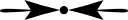
\includegraphics[width=2cm]{figures/div1}
%\end{center}
%\vfill

\newpage

\begin{center}
\Large Jetzt noch Etwas über das Fachinger Wasser\par
\end{center}

Im Anfang erinnerte ich,
daß das Fachinger Wasser noch zu wenig bei unseren Landsleuten bekannt,
und selbst noch vielen unsern Doktoren fremd sei,
indem dasselbe außer [in] einigen großen Städten, nicht zu haben ist,
welches doch um seinen mannigfaltigen großen Nutzen äußerst zu beklagen,
und vielleicht der Art und Weise,
wie man dasselbe bekannt gemacht hat,
zuzuschreiben ist, welches wir nicht weiter untersuchen wollen.
Im Jahre 1791 ist unter andern eine Abhandlung darüber
bei dem Buchhändler van Cleef im Haag%
\footnoteA{Unter dem Titel:
\emph{Beschreibung des Fachinger Mineralwassers
und seiner heilsamen Wirkungen}
von M. G. Thilenius,
Dr. in der Arzneiwissenschaft
und Mitgliede der Chur-Männischen Akademie der Wissenschaften.}
unentgeltlich ausgegeben worden,
welches eine Übersetzung eines deutschen Werkchens
des Hrn. Dr. Thilenius war,
worin die Vollkommenheiten dieses Wassers dargestellt wurden.
Weiter sind von Zeit zu Zeit in deutscher Sprache Berichte erschienen,
die einen kurzen Auszug aus bemeldeter Abhandlung in sich enthielten,
welche indessen,
obschon man alles Lob den Tugenden dieses Wassers schuldig ist,
in ihrer Erhebung ein wenig zu weit gehen.
Da ich dennoch durch meine eigene angestellten Proben
von dem außerordentlichen Wert dieses Wassers überzeugt bin,
und auch von einem jeden,
der seine Bestandteile untersuchen und prüfen will,
als ein solches wird befunden werden;
so glaube ich,
meinen Landsleuten mit der Übersetzung von einem der kleinen Berichte,
welche mir als der beste bekannt,
und von nachfolgendem Inhalt ist,
einen wesentlichen Dienst zu erweisen.

\vfill
\begin{center}
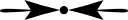
\includegraphics[width=2cm]{figures/div1}
\end{center}
\vfill

\newpage
\fancyhead[C]{=\kern-0.14em=\kern-0.14em=\kern-0.14em=\kern-0.14em= \thepage\kern+0.14em =\kern-0.14em=\kern-0.14em=\kern-0.14em=\kern-0.14em=}
{\centering
    {\Large Nachricht an das Publikum,}\\
    {\small das}\\
    \vspace{.5em}
    {\LARGE Fachinger Mineralwasser}\\
    {\small betreffend.}\\

    \begin{center}\begin{minipage}{4cm}
      \centering
      \hrulefill\\
    \end{minipage}\end{center}
}

\lettrine{S}o wenig das jetzt eben so bekannt -
als [das] geschätzte Fachinger Mineralwasser
noch einer weiteren Empfehlung bei Ärzten bedarf,
und jedem dessen nicht gemeine Kräfte,
die dasselbe mit einer ihm ganz vorzüglichen Annehmlichkeit verbindet,
durch die Beschriebung von Herrn Dr. Thilenius bekannt sind;
so wollen wir nun das Publikum
auf einige diesem Mineralwasser vorzüglichen Heilkräfte
von Zeit zu Zeit aufmerksam machen. -
Für jetzt nur einiges:\\

1) Bei den sogenannten Gallen- und Faulfiebern
zeigt sich dieses Wasser durch Linderung
der gewöhnlich damit verbundenen heftigen Kopfschmerzen,
des unerträglichen Duftes,
des oft mit Schmerzen abgehenden Urins,
und überhaupt der damit verbundenen allgemeinen Fieberhitze,
ungemein heilsam.
Bei häufigem Erbrechen in diesem Fieber,
kenne ich kein angenehmeres und mehr erquickendes Mittel,
als das Fachinger Wasser mit Zitronensaft und etwas Zucker versüßt.
Mehrere arme Kranke,
die dieses Jahr das in unserer Gegend
so ausgebreitet herrschende sehr ansteckende Nervenfieber hatten,
wurden, nach vorher sorgfältig gereinigtem Magen,
durch dieses Mineralwasser mit Eßigsirup vermischt,
und im Aufbrausen getrunken, hergestellt.
Kennt man den großen Nutzen,
den vorzüglich englische Ärzte
zuerst von der fixen Luft in diesen Krankheiten beobachteten;
so läßt sich der Nutzen
des mit dieser Luftsäure so sehr reichlich gesättigten Fachinger Wassers
leicht einsehen.\\

2) In hysterischen und hypochondrischen Krämpfen, Vapeurs%
\footnoteB{\cftext Blähungen},
Mutterbeschwerden,
die durch krampfhaftes Auftreiben des Magens und der Gedärme,
durch Herzklopfen, überhingehende Hitze des Gesichts,
saures Aufbrausen%
\footnoteB{\cftext Aufstoßen},
durch Erbrechen einer sauren grünen Galle u.s.w. befallen,
schafft dieses Mineralwasser
durch Tilgung des Reizes im Magen oft  augenblicklichen Nutzen,
und besser, als Krebssteine%
\footnoteB{\cftext Krebssteine bestehen
vor allem aus Kalk- und Magnesiumsalzen
und wurden früher zu Magen- und Zahnpulver verarbeitet.
(Quelle: https://www.wissen.de/lexikon/krebssteine)},
und die so häufig mißbrauchte weiße Magnesie%
\footnoteB{\cftext Bittersalzerde, Magnesiumoxid}
u. d. gl. Nüchtern eine Zeit lang entwelche Gläser von diesem Wasser,
z.B. den dritten Teil eines Krugs getrunken,
verbessert [es] auf eine sanfte Weise die Anlage
zu diesem jetzt fast zur Mode gewordenen krampfhaften Übel,
so wie dieses Mineralwasser bei Magensäure,
dem daher rührenden Sodbrennen und Magenschmerzen,
aber dem Kopfweh nach einer kleinen Weinfreude unübertreffbar ist,
und in diesen Fällen mehrentheils
durch Erzeugung eines gelinden Durchfalls
den Feind aus dem Leibe schafft.\\

3) Kinder, die bei einem dicken mit saurem schleimausgetropften Unterleib,
an sogenannten Wurm-Zufällen leiden,
und bei denen oft ein gehöriger Gebrauch
von  Arzneimitteln nicht anzubringen ist,
werden öfters durch reichliches Trinken dieses Wassers völlig hergestellt,
und der bei Zufällen oft aufgehaltene Wachstum der Kinder
nachher sichtbar und auffallend befördert.
Überhaupt kenne ich kein Mittel,
das bei langwierigen schleichenden Kinderkrankheiten,
die so sehr mit schleimigen Stockungen
in den Drüsen des Unterleibes verbunden sind,
ein angenehmeres, und den mehresten Kindern mehr behangendes,
viel wirkendes Mittel wäre,
als unser Fachinger Wasser,
wenn dessen Säure tilgende, Schleim auflösende,
und dabei durch sein flüchtigen Eisenstoff
die Eingeweide sanft stärkende Kräfte,
lange und gehörig benutzt werden.
Vielleicht über dessen richtigen Gebrauch ein anderes Mal.\\
\\

\hfill
\begin{minipage}{6cm}
  \centering
{\Large Fried. Diel,}\\
Physicus in Dietz und Doctor\\
im Baad Embs.
\end{minipage}

\vfill
\begin{center}
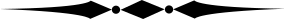
\includegraphics[width=4cm]{figures/div2}
\end{center}
\vfill%
%
% if pagenumber uneven, make newpage
\checkoddpage\ifoddpage
  \newpage\strut
  \fancyhead[C]{}\fi

\end{document}
